\chapter[Atmel STK500/1 Board]{Atmel STK500/1 Board}

\section{Introduction}

This chapter describes the support done in \ee\ for the
Atmel STK500/1 Board (see Figure \ref{fig:stk500-501}).

\begin{figure}
  \begin{center}
    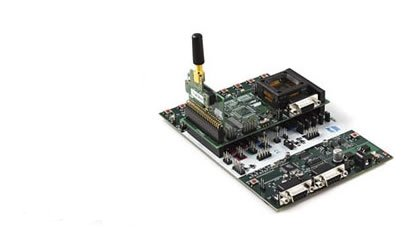
\includegraphics[width=6cm, bb=0 0 402 228]{images/atmel_zig.jpg}
  \end{center}
  \caption{The Atmel STK500/1 board running \ee.}
  \label{fig:stk500-501}
\end{figure}

The STK500/1 is a low cost, efficient development board produced by
Atmel with interfaces to JTAG, SPI, and RS-232 \cite{atmelZigbee}.

To configure the usage of the STK500/1 Board, the user has to specify an
appropriate \const{BOARD_DATA}, as in the following example:

\begin{lstlisting}
  ...
  BOARD_DATA = ATMEL_STK50X {
    ...
  }
  ...
\end{lstlisting}

The STK500/1 board supports a set of devices which are directly
available and mounted on it. These devices can be configured by adding
attributes inside the \const{BOARD_DATA} section.

The supported devices and the API functions needed to use them are
described in the following sections.

Please note that the current version of the board support only
supports the \avr\ model ATMEGA128.

Please remember that you have to connect ISP6PIN plug of the STK500
with the SPROG plug of the STK501 through 6-wires cable.


% -------------------------------------------------------------------

\section{LEDs}

The Atmel STK500 Board has a set of 8 LEDs attached to the PORTB pins
of the microcontroller. To use the LEDs on the Board, the developer
should specify the \const{USELEDS} attribute as TRUE, as in the
following example:

\begin{lstlisting}
  ...
  BOARD_DATA = ATMEL_STK50X {
    USELEDS = TRUE;
    ...
  }
  ...
\end{lstlisting}

The following subsections will describe the functions available to
control the Atmel STK500 LEDs.


\begin{function_nopb2}{EE\_led\_1\_on}{EE_led_1_on:stk50x}
  \synopsis{void EE_led_1_on(void);}
  
  \begin{fundescription}
    The function turns on LED 1.
  \end{fundescription}
  
%  \begin{funparameters}
%    \fpar{none}{None in this function.}
%  \end{funparameters}
  
%  \begin{funreturn}
%    \fret{void}{The function does not return a value.}
%  \end{funreturn}
  
%  \begin{funconformance}
%  \end{funconformance}
\end{function_nopb2}

\begin{function_nopb2}{EE\_led\_1\_off}{EE_led_1_off:stk50x}
  \synopsis{void EE_led_1_off(void);}
  
  \begin{fundescription}
    The function turns off LED 1.
  \end{fundescription}
  
%  \begin{funparameters}
%    \fpar{none}{None in this function.}
%  \end{funparameters}
  
%  \begin{funreturn}
%    \fret{void}{The function does not return a value.}
%  \end{funreturn}
  
%  \begin{funconformance}
%  \end{funconformance}
\end{function_nopb2}

\begin{function_nopb2}{EE\_led\_2\_on}{EE_led_2_on:stk50x}
  \synopsis{void EE_led_2_on(void);}
  
  \begin{fundescription}
    The function turns on LED 2.
  \end{fundescription}
  
%  \begin{funparameters}
%    \fpar{none}{None in this function.}
%  \end{funparameters}
  
%  \begin{funreturn}
%    \fret{void}{The function does not return a value.}
%  \end{funreturn}
  
%  \begin{funconformance}
%  \end{funconformance}
\end{function_nopb2}

\begin{function_nopb2}{EE\_led\_2\_off}{EE_led_2_off:stk50x}
  \synopsis{void EE_led_2_off(void);}
  
  \begin{fundescription}
    The function turns off LED 2.
  \end{fundescription}
  
%  \begin{funparameters}
%    \fpar{none}{None in this function.}
%  \end{funparameters}
  
%  \begin{funreturn}
%    \fret{void}{The function does not return a value.}
%  \end{funreturn}
  
%  \begin{funconformance}
%  \end{funconformance}
\end{function_nopb2}

\begin{function_nopb2}{EE\_led\_3\_on}{EE_led_3_on:stk50x}
  \synopsis{void EE_led_3_on(void);}
  
  \begin{fundescription}
    The function turns on LED 3.
  \end{fundescription}
  
%  \begin{funparameters}
%    \fpar{none}{None in this function.}
%  \end{funparameters}
  
%  \begin{funreturn}
%    \fret{void}{The function does not return a value.}
%  \end{funreturn}
  
%  \begin{funconformance}
%  \end{funconformance}
\end{function_nopb2}

\begin{function_nopb2}{EE\_led\_3\_off}{EE_led_3_off:stk50x}
  \synopsis{void EE_led_3_off(void);}
  
  \begin{fundescription}
    The function turns off LED 3.
  \end{fundescription}
  
%  \begin{funparameters}
%    \fpar{none}{None in this function.}
%  \end{funparameters}
  
%  \begin{funreturn}
%    \fret{void}{The function does not return a value.}
%  \end{funreturn}
  
%  \begin{funconformance}
%  \end{funconformance}
\end{function_nopb2}

\begin{function_nopb2}{EE\_led\_4\_on}{EE_led_4_on:stk50x}
  \synopsis{void EE_led_4_on(void);}
  
  \begin{fundescription}
    The function turns on LED 4.
  \end{fundescription}
  
%  \begin{funparameters}
%    \fpar{none}{None in this function.}
%  \end{funparameters}
  
%  \begin{funreturn}
%    \fret{void}{The function does not return a value.}
%  \end{funreturn}
  
%  \begin{funconformance}
%  \end{funconformance}
\end{function_nopb2}

\begin{function_nopb2}{EE\_led\_4\_off}{EE_led_4_off:stk50x}
  \synopsis{void EE_led_4_off(void);}
  
  \begin{fundescription}
    The function turns off LED 4.
  \end{fundescription}
  
%  \begin{funparameters}
%    \fpar{none}{None in this function.}
%  \end{funparameters}
  
%  \begin{funreturn}
%    \fret{void}{The function does not return a value.}
%  \end{funreturn}
  
%  \begin{funconformance}
%  \end{funconformance}
\end{function_nopb2}

\begin{function_nopb2}{EE\_led\_5\_on}{EE_led_5_on:stk50x}
  \synopsis{void EE_led_5_on(void);}
  
  \begin{fundescription}
    The function turns on LED 5.
  \end{fundescription}
  
%  \begin{funparameters}
%    \fpar{none}{None in this function.}
%  \end{funparameters}
  
%  \begin{funreturn}
%    \fret{void}{The function does not return a value.}
%  \end{funreturn}
  
%  \begin{funconformance}
%  \end{funconformance}
\end{function_nopb2}

\begin{function_nopb2}{EE\_led\_5\_off}{EE_led_5_off:stk50x}
  \synopsis{void EE_led_5_off(void);}
  
  \begin{fundescription}
    The function turns off LED 5.
  \end{fundescription}
  
%  \begin{funparameters}
%    \fpar{none}{None in this function.}
%  \end{funparameters}
  
%  \begin{funreturn}
%    \fret{void}{The function does not return a value.}
%  \end{funreturn}
  
%  \begin{funconformance}
%  \end{funconformance}
\end{function_nopb2}

\begin{function_nopb2}{EE\_led\_6\_on}{EE_led_6_on:stk50x}
  \synopsis{void EE_led_6_on(void);}
  
  \begin{fundescription}
    The function turns on LED 6.
  \end{fundescription}
  
%  \begin{funparameters}
%    \fpar{none}{None in this function.}
%  \end{funparameters}
  
%  \begin{funreturn}
%    \fret{void}{The function does not return a value.}
%  \end{funreturn}
  
%  \begin{funconformance}
%  \end{funconformance}
\end{function_nopb2}

\begin{function_nopb2}{EE\_led\_6\_off}{EE_led_6_off:stk50x}
  \synopsis{void EE_led_6_off(void);}
  
  \begin{fundescription}
    The function turns off LED 6.
  \end{fundescription}
  
%  \begin{funparameters}
%    \fpar{none}{None in this function.}
%  \end{funparameters}
  
%  \begin{funreturn}
%    \fret{void}{The function does not return a value.}
%  \end{funreturn}
  
%  \begin{funconformance}
%  \end{funconformance}
\end{function_nopb2}

\begin{function_nopb2}{EE\_led\_7\_on}{EE_led_7_on:stk50x}
  \synopsis{void EE_led_7_on(void);}
  
  \begin{fundescription}
    The function turns on LED 7.
  \end{fundescription}
  
%  \begin{funparameters}
%    \fpar{none}{None in this function.}
%  \end{funparameters}
  
%  \begin{funreturn}
%    \fret{void}{The function does not return a value.}
%  \end{funreturn}
  
%  \begin{funconformance}
%  \end{funconformance}
\end{function_nopb2}

\begin{function_nopb2}{EE\_led\_7\_off}{EE_led_7_off:stk50x}
  \synopsis{void EE_led_7_off(void);}
  
  \begin{fundescription}
    The function turns off LED 7.
  \end{fundescription}
  
%  \begin{funparameters}
%    \fpar{none}{None in this function.}
%  \end{funparameters}
  
%  \begin{funreturn}
%    \fret{void}{The function does not return a value.}
%  \end{funreturn}
  
%  \begin{funconformance}
%  \end{funconformance}
\end{function_nopb2}

\begin{function_nopb2}{EE\_led\_8\_on}{EE_led_8_on:stk50x}
  \synopsis{void EE_led_8_on(void);}
  
  \begin{fundescription}
    The function turns on LED 8.
  \end{fundescription}
  
%  \begin{funparameters}
%    \fpar{none}{None in this function.}
%  \end{funparameters}
  
%  \begin{funreturn}
%    \fret{void}{The function does not return a value.}
%  \end{funreturn}
  
%  \begin{funconformance}
%  \end{funconformance}
\end{function_nopb2}

\begin{function_nopb2}{EE\_led\_8\_off}{EE_led_8_off:stk50x}
  \synopsis{void EE_led_8_off(void);}
  
  \begin{fundescription}
    The function turns off LED 8.
  \end{fundescription}
  
%  \begin{funparameters}
%    \fpar{none}{None in this function.}
%  \end{funparameters}
  
%  \begin{funreturn}
%    \fret{void}{The function does not return a value.}
%  \end{funreturn}
  
%  \begin{funconformance}
%  \end{funconformance}
\end{function_nopb2}


% -------------------------------------------------------------------


